% 05_results.tex  --  Results

\section{Results}
\label{sec:results}

\subsection{Does the Landscape Predict Performance?}
\label{sec:results-ordering}

Method-level split-regret ranks method families in the small-to-mid-size
benchmark (\Cref{fig:universal,tab:allmethods}). The score is computed before
candidate retraining and is strongly monotone with eventual AUROC at the
method-mean level: gain-path methods sit in the low-regret/high-AUROC corner,
while the coverage-optimal HD-Greedy method sits at the opposite extreme.
Gradient sampling is the main exception, and the decomposition below shows why:
its problem is leaf-value estimation, not split-structure preservation. This
17-method diagnostic grid uses 26 datasets, two audited budgets, and three
seeds, and is separate from the five-budget, five-seed core grid in
\Cref{tab:headline}. The large-scale audit in \cref{sec:results-scale} bounds
the claim: once high-gain margins are cleared on very large datasets, root
split-regret loses rank resolution.

% ---- Figure 2: Universal SLD map (headline) ----
\begin{figure}[!t]
\centering
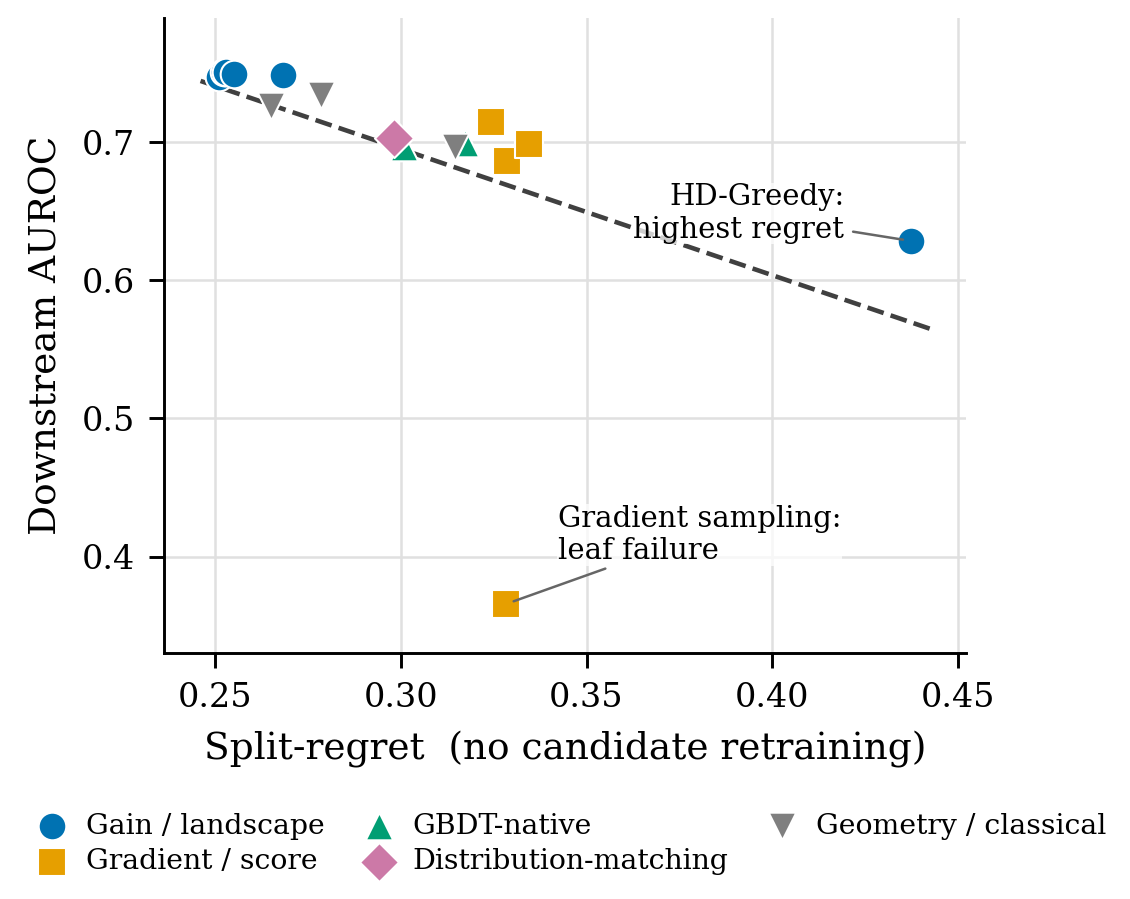
\includegraphics[width=\columnwidth]{figures/fig_c1_universal.png}
\caption{%
  \textbf{No-candidate-retraining method audit.}
  Each point is one condensation method. Lower split-regret, computed before
  candidate retraining, tracks higher downstream AUROC over 156
  dataset--budget--seed cells (Spearman $\rho=-0.87$, OLS slope $-0.91$).%
}
\label{fig:universal}
\end{figure}

% ---- Table 2: Headline performance + fidelity ----
\begin{table}[!t]
\centering
\caption{Headline performance and diagnostics for five core methods (3,250 cells).
AUROC uses mean$\pm$95\% CI over dataset clusters; avg.\ rank lower is better.
Raw SLD$_\infty$ is diagnostic only and is not a cross-dataset fidelity score;
speedup is relative to full-data retraining on the same dataset/learner.}
\label{tab:headline}
\scriptsize
\setlength{\tabcolsep}{3pt}
\begin{tabular}{@{}lcccc@{}}
\toprule
\textbf{Method} & \textbf{AUROC} & \textbf{Rank} &
  \textbf{Raw SLD}$_\infty$ \textbf{diag.} & \textbf{Speedup} \\
\midrule
Full data & $0.812 \pm 0.062$ & -- & -- & 1.0$\times$ \\
Legacy gain-path  & $0.743 \pm 0.057$ & 2.60 & 99.4  & 3.9$\times$ \\
HistDistill-Refined  & $0.742 \pm 0.057$ & 2.68 & 93.6 & 3.5$\times$ \\
HistDistill-Density  & $0.742 \pm 0.057$ & 2.65 & 93.7 & 3.5$\times$ \\
Herding           & $0.731 \pm 0.054$ & 3.44 & 174.1  & 3.8$\times$ \\
Random            & $0.724 \pm 0.056$ & 3.63 & 138.3  & 4.0$\times$ \\
\bottomrule
\end{tabular}
\end{table}

The gradient-sampling AUROC is an audited failure mode rather than a plotting
artifact: its deployed AUROC is also low in the reference-chain subset
(\Cref{tab:decomp}), where the error is leaf-estimate dominated. The
method-level association is not driven only by this point or by HD-Greedy:
excluding both leaves Spearman $\rho=-0.85$ over the remaining 15 methods.

% ---- Table 3: Universal 17-method audit ----
\begin{table}[!t]
\centering
\caption{Seventeen-method diagnostic audit. Values are method means
$\pm$95\% CI over dataset clusters, over 156 dataset--budget--seed cells.
Lower split-regret and higher AUROC are better. EL2N and GraNd coincide after
rounding under the fixed-state adaptation used here.}
\label{tab:allmethods}
\tiny
\setlength{\tabcolsep}{2.5pt}
\begin{tabular}{@{}lrr@{}}
\toprule
\textbf{Method} & \textbf{AUROC} & \textbf{Regret} \\
\midrule
Gain-path sketch & $0.748\pm0.062$ & $0.251\pm0.079$ \\
Legacy gain-path & $0.751\pm0.062$ & $0.252\pm0.079$ \\
HD-Density & $0.751\pm0.061$ & $0.253\pm0.073$ \\
HD-Refined & $0.750\pm0.062$ & $0.255\pm0.077$ \\
Random & $0.726\pm0.060$ & $0.265\pm0.064$ \\
Gain sketch & $0.749\pm0.062$ & $0.268\pm0.081$ \\
Herding & $0.734\pm0.059$ & $0.279\pm0.082$ \\
DM & $0.703\pm0.062$ & $0.298\pm0.075$ \\
MVS & $0.697\pm0.058$ & $0.301\pm0.068$ \\
K-center & $0.697\pm0.062$ & $0.315\pm0.079$ \\
GOSS & $0.700\pm0.058$ & $0.317\pm0.073$ \\
GradMatch & $0.715\pm0.057$ & $0.324\pm0.086$ \\
Grad.\ samp. & $0.366\pm0.067$ & $0.328\pm0.078$ \\
EL2N & $0.686\pm0.056$ & $0.329\pm0.071$ \\
GraNd & $0.686\pm0.056$ & $0.329\pm0.071$ \\
CRAIG & $0.699\pm0.061$ & $0.335\pm0.082$ \\
HD-Greedy & $0.629\pm0.050$ & $0.437\pm0.106$ \\
\bottomrule
\end{tabular}
\end{table}

Negative leaf gaps mean deployed condensed leaves slightly outperform the
full-data leaf refit under this diagnostic chain, usually through regularisation
or favourable condensed weighting.

Lower raw SLD predicts higher AUROC within a dataset, but pooling across
datasets is confounded (\Cref{fig:sldlaw}). Within each dataset, lower raw
$\delta_\infty$ corresponds to better retrained AUROC; after pooling datasets,
the trend can invert because dataset scale affects both raw SLD magnitude and
absolute AUROC. Raw SLD should therefore be used for within-dataset,
within-budget method comparison, not as a cross-dataset absolute score.

% ---- Figure 3: SLD law scatter ----
\begin{figure}[!t]
\centering
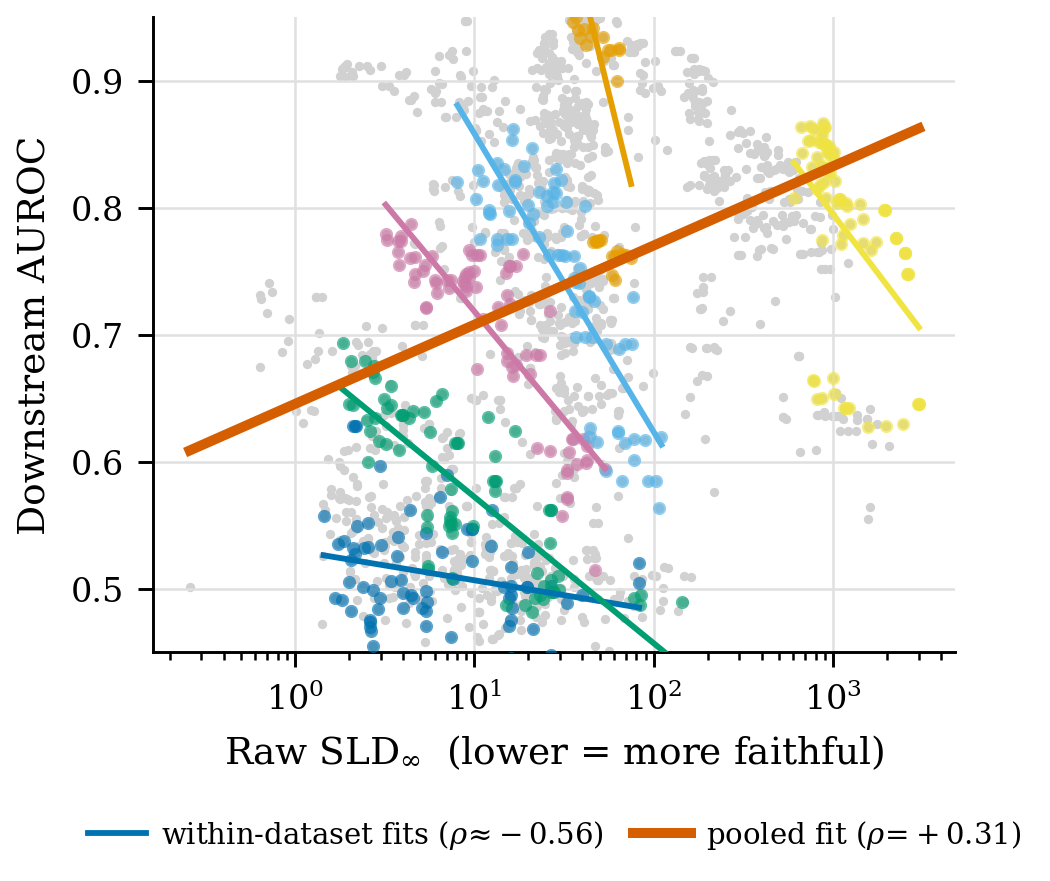
\includegraphics[width=\columnwidth]{figures/fig_c2_sldlaw.png}
\caption{%
  \textbf{Within-dataset SLD trend.}
  Coloured lines are within-dataset fits on log-scale raw SLD; the average
  within-dataset trend is negative. The pooled fit reverses because dataset
  scale confounds raw SLD and AUROC.%
}
\label{fig:sldlaw}
\end{figure}

\subsection{Coverage Is Not Predictive Fidelity}
\label{sec:results-coverage}

The near-optimal coverage selector is weak by downstream predictive
performance (\Cref{fig:coverage,tab:coverage}). HD-Greedy optimises
split-threshold coverage and achieves the expected coverage win, but this
objective is not the one that preserves downstream AUROC. The method lands in
the bottom tier of the 17-method audit (\Cref{tab:allmethods}); unweighted
threshold coverage and gain-weighted landscape fidelity are different
objectives.

% ---- Figure 4: Selector coverage ----
\begin{figure}[!t]
\centering
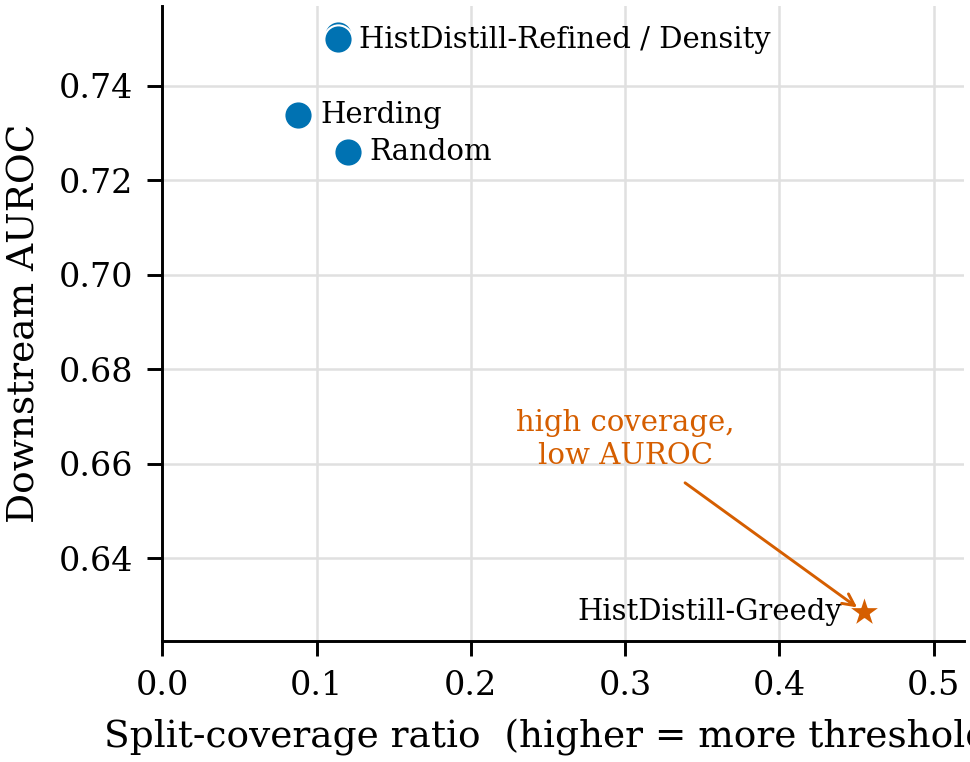
\includegraphics[width=\columnwidth]{figures/fig_c3_coverage.png}
\caption{%
  \textbf{Coverage is not predictive fidelity.}
  HD-Greedy covers the most high-gain split thresholds, but the accurate
  methods occupy a different region of the coverage--AUROC plane.%
}
\label{fig:coverage}
\end{figure}

% ---- Coverage paradox table ----
\begin{table}[!t]
\centering
\caption{Coverage metrics versus AUROC on the two-budget coverage audit.
Cov. is high-gain split coverage; Proxy is coverage divided by the proxy upper
bound.}
\label{tab:coverage}
\scriptsize
\setlength{\tabcolsep}{2pt}
\begin{tabular}{@{}lrrrrr@{}}
\toprule
\textbf{Method} & \textbf{Cov25} & \textbf{Proxy25} &
  \textbf{Cov50} & \textbf{Proxy50} & \textbf{AUROC} \\
\midrule
HD-Greedy & 0.371 & 1.000 & 0.539 & 1.000 & 0.629 \\
Random & 0.082 & 0.246 & 0.159 & 0.299 & 0.726 \\
HD-Refined & 0.075 & 0.223 & 0.152 & 0.286 & 0.750 \\
HD-Density & 0.075 & 0.223 & 0.152 & 0.286 & 0.751 \\
Herding & 0.059 & 0.183 & 0.118 & 0.229 & 0.734 \\
\bottomrule
\end{tabular}
\end{table}

The decomposition shows that the coverage failure is structural, whereas
gradient sampling fails for a different reason (\Cref{fig:decomp,tab:decomp}).
The reference chain separates structure error from leaf-estimate gap.
HD-Greedy's loss comes from choosing the wrong gain-weighted structure, not from
poor leaf values after its structure is fixed. Gradient sampling is the
opposite diagnostic case: its population mismatch is low, but its leaf-estimate
gap is high, pointing to distorted within-leaf gradient/Hessian or reweighting
statistics.

% ---- Figure 5: Error decomposition ----
\begin{figure}[!t]
\centering
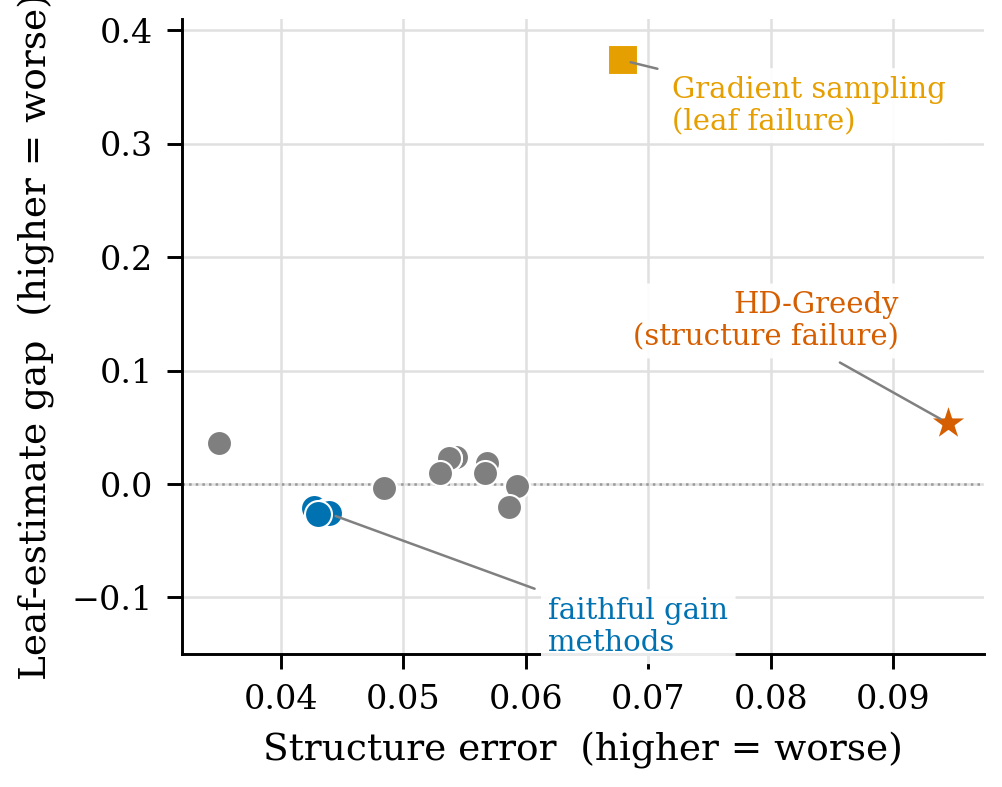
\includegraphics[width=\columnwidth]{figures/fig_c4_decomp.png}
\caption{%
  \textbf{Two failure modes.}
  HD-Greedy is structure-dominated; gradient sampling is leaf-estimate dominated.
  Faithful gain methods occupy the low-error corner.%
}
\label{fig:decomp}
\end{figure}

% ---- Decomposition table ----
\begin{table}[!t]
\centering
\caption{Error decomposition on the diagnostic subset used to illustrate both
failure modes. Absolute AUROCs differ from the pooled values in
\Cref{tab:headline,fig:universal}. Structure error is reference minus leaf-refit;
leaf gap is leaf-refit minus deployed.}
\label{tab:decomp}
\scriptsize
\setlength{\tabcolsep}{2.5pt}
\begin{tabular}{@{}lrrrrr@{}}
\toprule
\textbf{Method} & \textbf{Dep.} & \textbf{Leaf} &
  \textbf{Str.\ Err} & \textbf{Leaf Gap} & \textbf{Pop.} \\
\midrule
HD-Greedy     & 0.643 & 0.696 & 0.094 & 0.054 & 0.243 \\
Grad.\ samp.  & 0.349 & 0.723 & 0.068 & 0.374 & 0.133 \\
DM            & 0.720 & 0.756 & 0.035 & 0.036 & 0.235 \\
K-center      & 0.713 & 0.737 & 0.054 & 0.024 & 0.196 \\
MVS           & 0.724 & 0.734 & 0.057 & 0.010 & 0.088 \\
GradMatch     & 0.734 & 0.732 & 0.059 & $-0.002$ & 0.113 \\
HD-Refined    & 0.773 & 0.747 & 0.044 & $-0.026$ & 0.060 \\
Legacy gp     & 0.774 & 0.748 & 0.043 & $-0.026$ & 0.068 \\
\bottomrule
\multicolumn{6}{@{}l@{}}{\scriptsize Decomposition-subset anchors: full AUROC $=0.826$, reference $=0.791$.}
\end{tabular}
\end{table}

\subsection{How Much Can Structure Be Perturbed?}
\label{sec:results-dose}

Calibrated split-gain noise exposes a margin-linked robustness pattern for GBDT
structure (\Cref{fig:dose,tab:dose}). AUROC and split agreement stay flat while
the margin condition in \eqref{eq:prop1} holds; beyond that point, agreement
drops first and AUROC degrades mildly. The result explains why aggressive
condensation can work when the dominant split margins are preserved, and why
corrupting high-gain structure is disproportionately costly.

% ---- Figure 6: Dose response ----
\begin{figure}[!t]
\centering
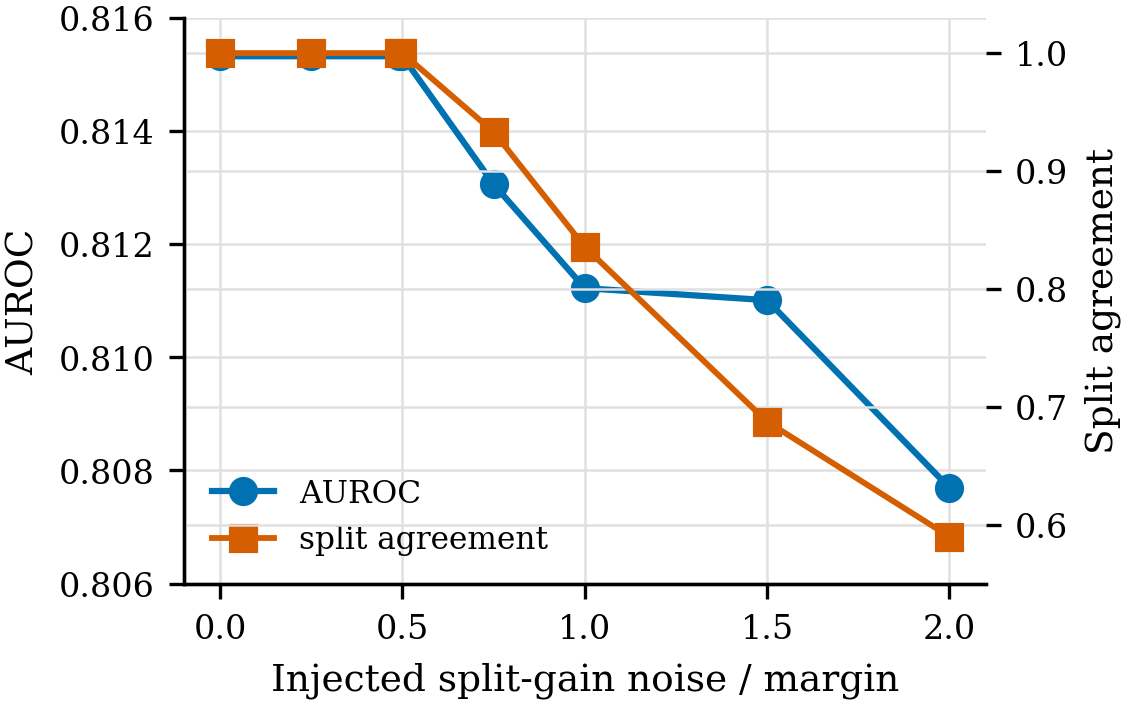
\includegraphics[width=\columnwidth]{figures/phase2_e18_downstream_dose_response.png}
\caption{%
  \textbf{Robustness pattern.}
  Split agreement drops after dose $0.5$; AUROC degrades mildly as calibrated
  split-gain noise exceeds the margin.%
}
\label{fig:dose}
\end{figure}

% ---- Dose response table ----
\begin{table}[!t]
\centering
\caption{Dose-response: 26 binary datasets, 1,872 cells. Values are
mean$\pm$95\% CI over dataset clusters; eight injected-noise levels are grouped
into five displayed rows.}
\label{tab:dose}
\scriptsize
\setlength{\tabcolsep}{3pt}
\begin{tabular}{@{}rcccc@{}}
\toprule
\textbf{Dose} & \textbf{AUROC} & \textbf{$\Delta$AUROC} &
  \textbf{Agree.} & \textbf{Regret} \\
\midrule
$\leq$0.50 & $0.815\pm0.068$ & 0.000 & $1.000\pm0.000$ & 0.000 \\
0.75 & $0.813\pm0.069$ & $-0.002$ & $0.933\pm0.002$ & 0.011 \\
1.00 & $0.811\pm0.069$ & $-0.004$ & $0.836\pm0.004$ & 0.030 \\
1.50 & $0.811\pm0.069$ & $-0.004$ & $0.687\pm0.008$ & 0.069 \\
2.00 & $0.808\pm0.070$ & $-0.008$ & $0.590\pm0.011$ & 0.101 \\
\bottomrule
\end{tabular}
\end{table}

\subsection{Performance, Fidelity, and Cost}
\label{sec:results-practical}

The top of the core grid is practically tied
(\Cref{tab:headline,tab:pairwise}). HistDistill-Refined and
HistDistill-Density match the legacy gain-path selector in AUROC while
achieving the lowest landscape discrepancy among the core methods. The
Refined-vs.-Legacy mean difference is operationally negligible and its
dataset-clustered confidence interval crosses zero. At the studied small-data
budgets, condensed retraining gives a median $3$--$4\times$ speedup, with
median condensed training under half a second in the recorded runs; SLD itself
costs one histogram pass.

\subsection{Does the Diagnostic Hold at Scale?}
\label{sec:results-scale}

\textbf{Scale audit: the cost payoff grows with $N$, while ordering is
dataset-dependent.}
A real large-data audit with 400-row condensed sets shows the payoff and the
limit of the diagnostic at deployment scale
(\Cref{fig:large-scale,tab:large-scale,tab:large-auroc}). Speedup rises from
single digits at $20$k rows to hundreds or thousands at million-row scale.
Random has the best large-$N$ AUROC point estimate on all three datasets, but
the three-dataset paired audit is underpowered (two-sided Wilcoxon $p=0.25$
vs.\ HD-Refined and HD-Density), so the practical reading is convergence among
reasonable condensers. This is the regime thesis: HD-Refined beats Random in
24/26 small-to-mid-size datasets (\Cref{tab:pairwise}), yet Random has the
largest point estimate on all three very large datasets
(\Cref{tab:large-auroc}).

HIGGS illustrates the same margin mechanism as \Cref{fig:sldlaw,fig:dose}:
several methods have zero root split-regret because the dominant root split is
saturated, so leaf estimates or deeper structure determine AUROC. Root-level
regret still rejects severe failures, but it cannot finely rank reasonable
surrogates once the top split margin is cleared.

\begin{figure}[!t]
\centering
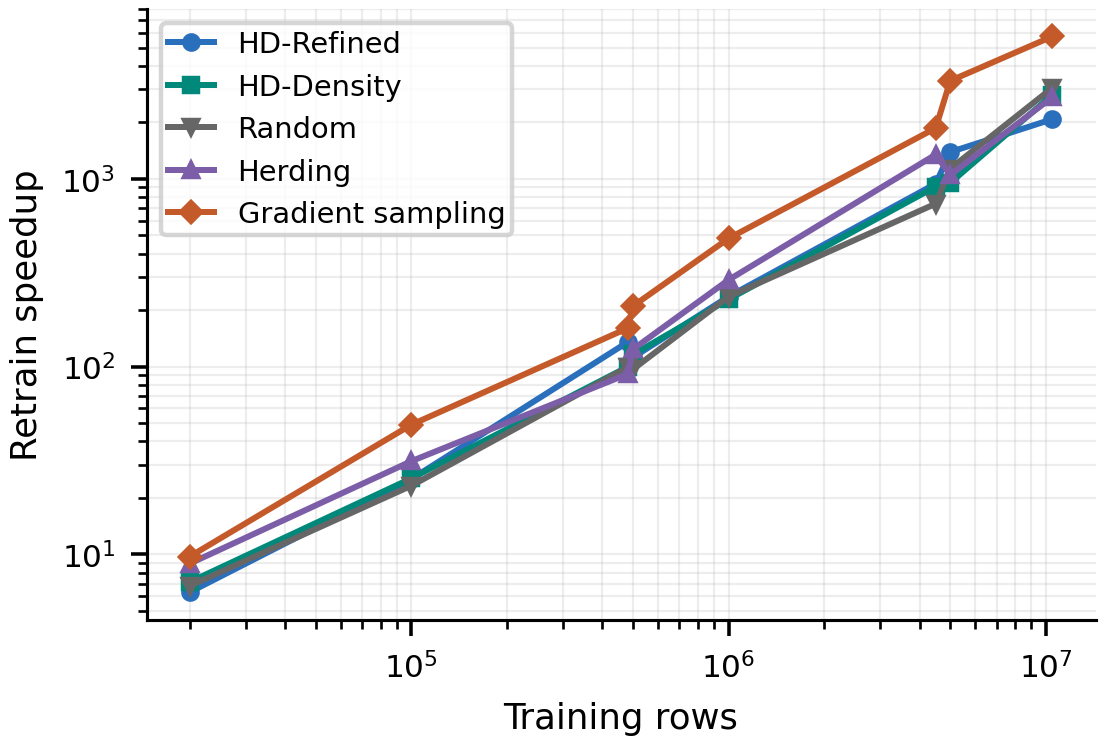
\includegraphics[width=\columnwidth]{figures/fig_large_scale_speedup.png}
\caption{%
  \textbf{Large-scale retraining payoff.}
  Log-log speedup for 400-row condensed retraining on Covertype, SUSY, and
  HIGGS. Points are single runs at observed dataset sizes, so no run-to-run CI
  is claimed for this scale audit.%
}
\label{fig:large-scale}
\end{figure}

\begin{table}[!t]
\centering
\caption{Large-scale audit at the largest training size per dataset. $\rho$ is
Spearman correlation over the five audited methods; negative $\rho$ means lower
split-regret aligns with higher AUROC. Each row is a single large-scale run.}
\label{tab:large-scale}
\scriptsize
\setlength{\tabcolsep}{3pt}
\begin{tabular}{@{}lrrr@{}}
\toprule
\textbf{Dataset} & \textbf{Rows} & $\boldsymbol{\rho}$ & \textbf{Top speedup} \\
\midrule
Covertype & 0.48M & $-0.36$ & $160\times$ \\
SUSY & 4.50M & $-0.97$ & $1{,}864\times$ \\
HIGGS & 10.50M & $0.11$ & $5{,}734\times$ \\
\bottomrule
\end{tabular}
\end{table}

\begin{table}[!t]
\centering
\caption{Large-scale AUROC at the largest training size. Full-data AUROCs are
0.897, 0.873, and 0.803 for Covertype, SUSY, and HIGGS. Random wins the
condensed point estimates, but the three-dataset paired audit is underpowered
($p=0.25$ against HD-Refined and HD-Density); no per-row CI is claimed because
the large-scale audit uses one full run per dataset/method.}
\label{tab:large-auroc}
\scriptsize
\setlength{\tabcolsep}{3pt}
\begin{tabular}{@{}lccc@{}}
\toprule
\textbf{Method} & \textbf{Cov.} & \textbf{SUSY} & \textbf{HIGGS} \\
\midrule
Full data & 0.897 & 0.873 & 0.803 \\
Random & \textbf{0.792} & \textbf{0.839} & \textbf{0.687} \\
HD-Refined & 0.747 & 0.818 & 0.648 \\
HD-Density & 0.781 & 0.794 & 0.641 \\
Herding & 0.719 & 0.780 & 0.450 \\
Grad.\ samp. & 0.377 & 0.219 & 0.364 \\
\bottomrule
\end{tabular}
\end{table}

\begin{figure}[!t]
\centering
\begin{tikzpicture}[
  font=\tiny,
  node distance=2mm,
  box/.style={rectangle, rounded corners=2pt, draw, align=center,
              text width=17mm, minimum height=7mm, inner sep=1.5pt},
  arr/.style={-Stealth, thick}
]
\node[box, fill=blue!8] (sld) {Compute SLD / split-regret};
\node[box, fill=red!8, right=of sld] (reject) {Reject high-regret failures};
\node[box, fill=green!8, right=of reject] (size) {Check scale and task};
\node[box, fill=yellow!12, below=of size] (small) {Small/mid $N$: prefer low-regret methods};
\node[box, fill=orange!12, above=of size] (large) {Very large $N$: choose fast reasonable surrogate};
\node[box, fill=gray!10, right=of size] (validate) {Validate HPO / regression on full data};
\draw[arr] (sld) -- (reject);
\draw[arr] (reject) -- (size);
\draw[arr] (size) -- (small);
\draw[arr] (size) -- (large);
\draw[arr] (size) -- (validate);
\end{tikzpicture}
\caption{%
  \textbf{Operational workflow implied by the measurements.}
  SLD is most useful as a cheap screening diagnostic: reject high-regret
  failures, prefer low-regret methods only when margins are not saturated, and
  validate HPO, regression, and final deployment choices on full data.%
}
\label{fig:workflow}
\end{figure}

% ---- Pairwise tests for core methods ----
\begin{table}[!t]
\centering
\caption{Dataset-clustered core-method comparisons. $\Delta$ is the paired mean
AUROC difference over 650 dataset--budget--seed cells; confidence intervals
bootstrap the 26 dataset clusters.}
\label{tab:pairwise}
\scriptsize
\setlength{\tabcolsep}{2.5pt}
\begin{tabular}{@{}llrrr@{}}
\toprule
\textbf{Method} & \textbf{Comparator} & $\boldsymbol{\Delta}$ &
  \textbf{95\% CI} & \textbf{DS wins} \\
\midrule
HD-Refined & Legacy gp & $-0.00056$ & [$-0.0019$, $0.0008$] & 11/26 \\
HD-Density & Legacy gp & $-0.00056$ & [$-0.0016$, $0.0005$] & 9/26 \\
HD-Refined & Herding & 0.01183 & [$0.0037$, $0.0204$] & 18/26 \\
HD-Refined & Random & 0.01807 & [$0.0124$, $0.0233$] & 24/26 \\
\bottomrule
\end{tabular}
\end{table}
